%%%%%%%%%%%%
%% Please rename this main.tex file and the output PDF to
%% [lastname_firstname_graduationyear]
%% before submission.
%%%%%%%%%%%%

\documentclass[12pt]{caltech_thesis}
\usepackage[hyphens]{url}
\usepackage{lipsum}
\usepackage{graphicx}
\usepackage{parskip}
\usepackage{layouts}
\setlength{\parindent}{2em} % Adjust '2em' to your preferred indent size
\usepackage{todonotes}
\newcommand{\tr}[1]{\textcolor{purple}{(TR:~#1)}} % Commenting

%% Tentative: newtx for better-looking Times
\usepackage[utf8]{inputenc}
\usepackage[T1]{fontenc}
\usepackage{newtxtext,newtxmath}

% Must use biblatex to produce the Published Contents and Contributions, per-chapter bibliography (if desired), etc.
\usepackage[
    backend=biber,natbib,
    % IMPORTANT: load a style suitable for your discipline
    style=authoryear
]{biblatex}

% Name of your .bib file(s)
\addbibresource{references.bib}
\addbibresource{ownpubs.bib}

\begin{document}

% Do remember to remove the square bracket!
\title{[Thesis Title]}
\author{Tom Röschinger}

\degreeaward{Ph.D. in Biochemistry and Molecuar Biophysics}                 % Degree to be awarded
\university{California Institute of Technology}    % Institution name
\address{Pasadena, California}                     % Institution address
\unilogo{caltech.png}                                 % Institution logo
\copyyear{2026}  % Year (of graduation) on diploma
\defenddate{xx/xx/2026}          % Date of defense

\orcid{0000-0002-4900-3216}

%% IMPORTANT: Select ONE of the rights statement below.
%\rightsstatement{All rights reserved\todo[size=\footnotesize]{Choose one from the choices in the source code!! And delete this \texttt{todo} when you're done that. :-)}}
% \rightsstatement{All rights reserved except where otherwise noted}
 \rightsstatement{Some rights reserved. This thesis is distributed under a MIT License.}
%%  If you'd like to remove the Caltech logo from your title page, simply remove the "[logo]" text from the maketitle command
\maketitle[logo]
%\maketitle

\begin{acknowledgements} 	 
   [Add acknowledgements here. If you do not wish to add any to your thesis, you may simply add a blank titled Acknowledgements page.]
\end{acknowledgements}

\begin{abstract}
   [This abstract must provide a succinct and informative condensation of your work. Candidates are welcome to prepare a lengthier abstract for inclusion in the dissertation, and provide a shorter one in the CaltechTHESIS record.]
\end{abstract}

%% Uncomment the `iknowhattodo' option to dismiss the instruction in the PDF.
% \begin{publishedcontent}%[iknowwhattodo]
% % List your publications and contributions here.
% %\nocite{Cahn:etal:2015}
% \end{publishedcontent}

\tableofcontents
\listoffigures
\listoftables
\printnomenclature

\mainmatter


\chapter{Introduction}
\begin{refsection}
\section{The great success of molecular biology}
\noindent For most of human history, the microbial world was limited to speculation and imagination.. That was until the late 17th century, when Antonie van Leeuwenhoek, a Dutch microscopist, was the first person to see microbes due to his exceptional skill in making single-lens microscopes~\citep{van1665observations,asimov1972asimov,lane2015unseen}. But it wasn't until the 19th century that Christian Gottfried Ehrenberg coined the word \textit{Bacterium} in 1828~\citep{ehrenberg1828symbolae} and Louis Pasteur disproved the theory of spontaneous generation~\citep{pasteur1862memoire}, the thought that life can commonly arise from non-living matter, and the study of bacteria became of broader interest. For the last two centuries, scientists from various backgrounds have studied the smallest forms of life as we know it. In 1885, Theodor Escherich discovered the bacterium \textit{Escherichia coli}~\citep{escherich1885darmbacterien}.
Since the isolation of its K12 strain, it has become one of the best-studied model organisms to date~\citep{bachmann1972pedigrees} and one of the greatest sources of groundbreaking and fundamental biological discoveries.

\indent Since the characterization of beta-D-galactosidase in 1950~\citep{lederberg1950beta}, the function of many genes in \textit{E. coli} K12 has been annotated. When its genome was fully sequenced for the first time in 1997, 4288 protein-coding open reading frames were identified~\citep{blattner1997complete} and genes were labeled by proposed function. Genes for which no function could be proposed either by previous work or by homology to genes with known function in other organisms were labeled with a \textit{y} as the first letter. The knowledge base of gene function in \textit{E. coli} has come so far, that it has become possible to simulate whole cell models of \textit{E. coli} cells and predict the abundance of a vast set of proteins and growth rates in a limited number of environmental conditions~\citep{sun2021coli}. The success of these predictive models relies on the fact that gene expression is not a stochastic free-for-all, but a tightly orchestrated process governed by specific regulatory logic.
%However, after 75 years of work, about one-third of \textit{E. coli}'s protein-coding sequences remain without functional annotation, a group of genes that has been coined the \textit{y-ome}~\citep{ghatak2019ome,moore2024revisiting}. In a 2016 study, the concentration of all proteins in \textit{E. coli} cells was measured in 22 different growth conditions. While the resulting data set is incredibly rich and powerful, it also shows that only about 58\% of genes account for more than 95\% of the protein mass in a cell.
\begin{figure}[hbt!]
\centering
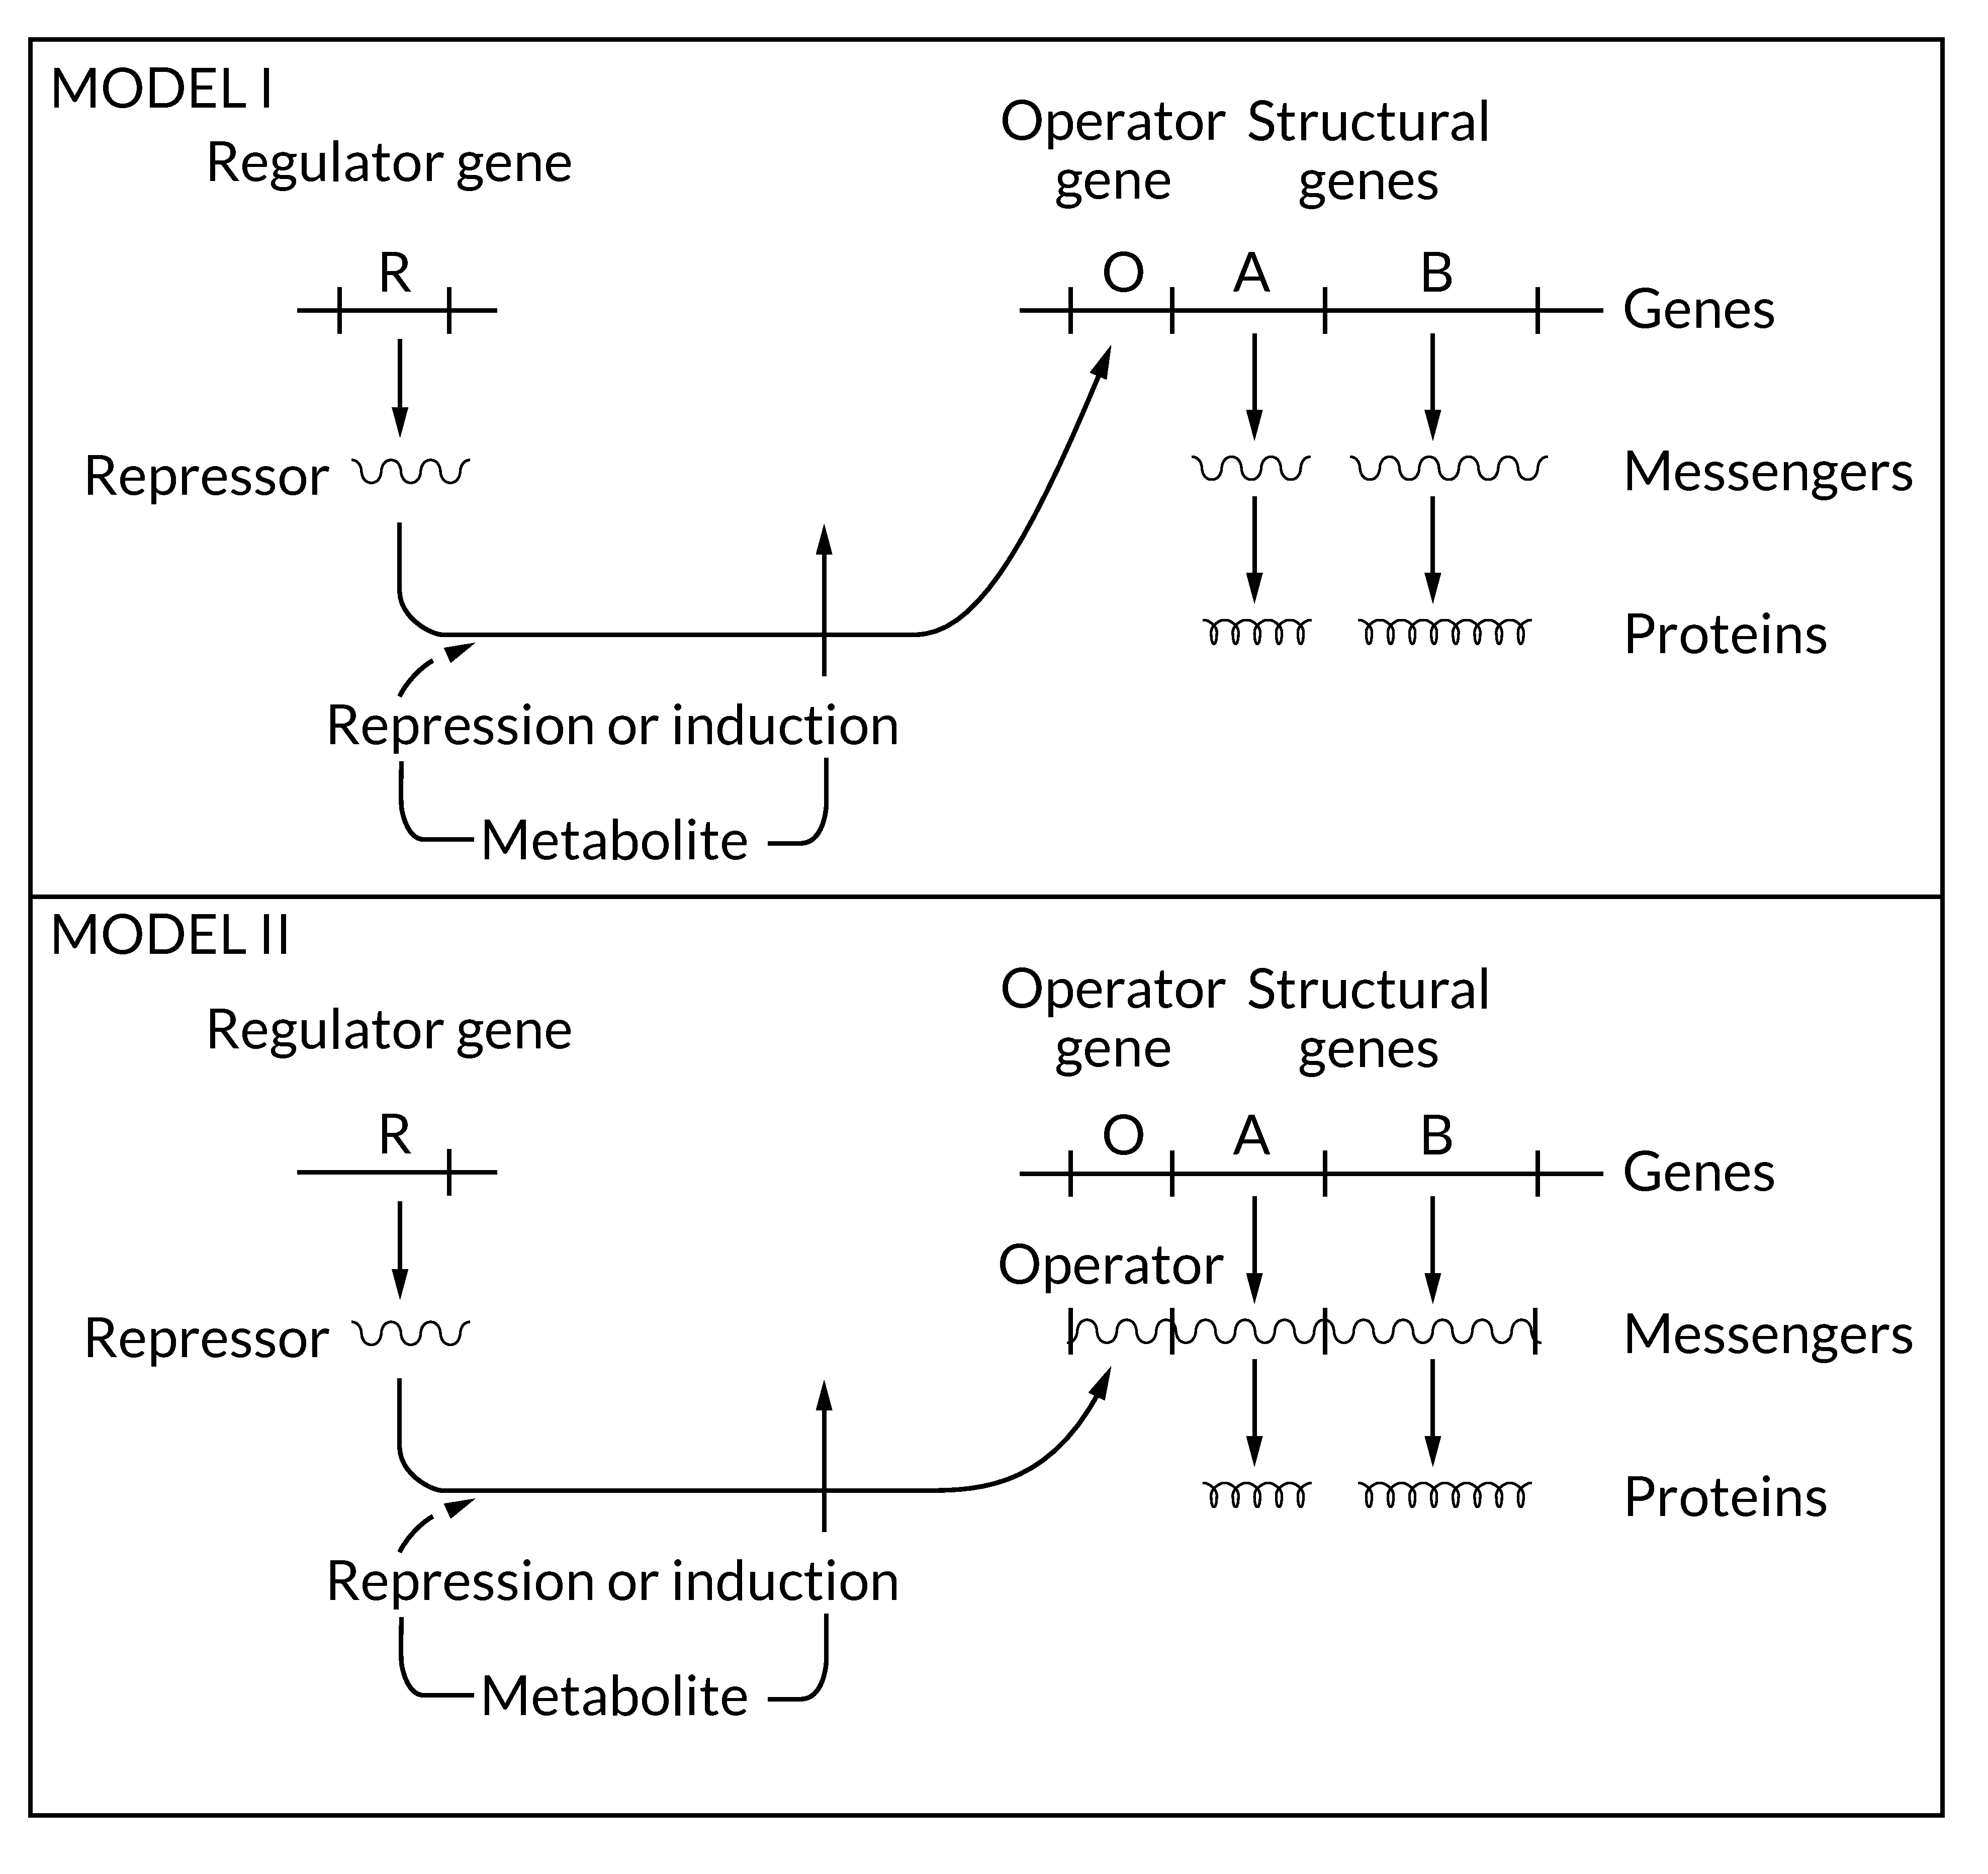
\includegraphics[width=.7\textwidth]{figures/intro/Jacob_Monod_fig6.pdf}
\caption[Discovery of gene regulation by Jacob and Monod.]{\textbf{Historical models of gene regulation in the lac operon.} Schematic representation of the two competing hypotheses proposed by Jacob and Monod: (Model 1) the genetic operator model, where the repressor acts directly on the DNA to inhibit transcription; and (Model 2) the cytoplasmic operator model, where regulation occurs at the level of the messenger RNA (translation). Kinetic evidence regarding mRNA stability ultimately favored Model 1. Adapted from \cite{jacob1961genetic}.}\label{fig:jacob_monod}
\index{figures}
\end{figure}\\
\indent In addition to identifying a gene's function, it is equally important to know when the gene is expressed. Fran{\c{c}}ois Jacob and Jacques Monod famously discovered the mechanism of repression and inducible expression of the lac-operon in 1961~\citep{jacob1961genetic}. While this work contains many more fundamental discoveries, such as the prediction of mRNA and its short lifetime and the refutation of the \textit{one gene, one enzyme} hypothesis, we focus on the discovery of the \textit{operon}. They found that a protein encoded in a different genomic location can control the expression of a set of genes by interacting with a piece of DNA. As shown in Figure~\ref{fig:jacob_monod}, Jacob and Monod discussed two possible models of repression, which they coined the "genetic operator model" (Model 1) and the "cytoplasmic operator model" (Model 2). In the genetic operator model, the repressor-operator interaction occurs at the genetic level, with the repressor directly controlling the synthesis of the gene. By considering the kinetics implied from this model, that the lifetime of the messenger molecule is short and that synthesis of the gene product should be stopped immediately once the gene is removed from the cell, this model was identified as the most likely. And as we now know, the lac repressor binds to DNA, inhibiting expression from the promoter of the lac operon by both sterically blocking binding of the RNA polymerase and by DNA looping, and the lifetimes of mRNA are on the order of minutes. \\
In the cytoplasmic operator model, the repressor binds to the messenger RNA, regulating its translation into protein. Jacob and Monod conclude that this model is unlikely because the size of RNA molecules it would require does not agree with the distributions of mRNA sizes measured at the time. Also, this model would require the messenger molecule to have much longer lifetimes. Jacob and Monod specifically noted that they could not disprove this model, and now we know that parts of it exist as small RNAs that can inhibit translation of mRNAs. It should also be noted that at the time of this work, neither the ribosome nor RNA polymerase had been discovered, which makes the discoveries and predictions Jacob and Monod proposed even more impressive.\\
\indent While Jacob and Monod established the fundamental logic of genetic switches, their work primarily focused on the existence of these regulatory interactions. In the decades that followed, the field shifted from identifying these "logic gates" to uncovering the precise molecular architectures that govern them. This transition revealed that regulation is often far more structurally complex than simple steric hindrance. As we will see, moving from a qualitative understanding to a predictive, quantitative theory requires both a detailed map of molecular geometry—such as that found in the \textit{ara} operon—and a physical framework to translate those geometries into mathematical functions. As will be explained below, it is fair to say that we both know a lot and at the same time very little about how genes are regulated in bacteria.
\begin{figure}[hbt!]
\centering
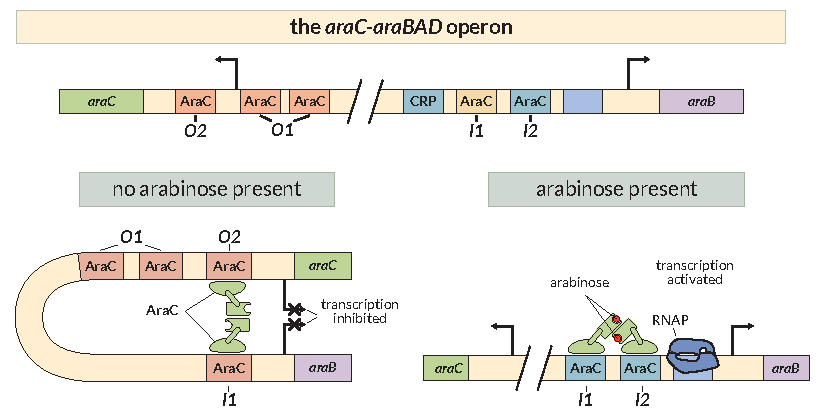
\includegraphics[width=\textwidth]{figures/intro/araB_operon_annotation.pdf}
\caption[Regulatory architecture of the araBAD operon.]{\textbf{Regulatory architecture of the araBAD operon.} (Left) In the absence of L-arabinose, the AraC homodimer binds to the distal \textit{I1} and \textit{O2} sites, forming a DNA loop that sterically hinders RNA polymerase binding at the.  Adapted from \cite{schleif2010arac}}\label{fig:araBAD}
\index{figures}
\end{figure}
\\ 
One of the best studied operons in \textit{E. coli} is the ara-operon, which was investigated in rigorous detail by the lab of Robert Schleif. This operon is responsible for the metabolism of L-arabinose and consists of the genes \textit{araBAD} and its divergently expressed regulator \textit{araC}~\citep{greenblatt1971arabinose}. As shown in Figure~\ref{fig:araBAD}, it was discovered that in the absence of L-arabinose, AraC forms a tetramer and binds to two distant binding sites (\textit{I1} and \textit{O2}), leading to the formation of a DNA loop, which suppresses expression from the promoters for \textit{araC} and \textit{araBAD}~\citep{dunn1984operator,martin1986dna,lobell1990dna}. If L-arabinose is present, it binds to each AraC dimer, leading to a conformational change and binding of the complex to the \textit{I1} and \textit{I2} binding sites in the \textit{araBAD} promoter. In this configuration, AraC initiates transcription, and arabinose is metabolised~\citep{schleif2010arac}.

\indent In addition to having a detailed understanding of molecular mechanisms for certain promoters, we have quantitative input-output functions for gene expression of promoters given variations in a diverse range of biophysical parameters. DNA-binding proteins often recognize specific DNA sequences as targets for binding, and the binding affinity is specific to those sequences. Using thermodynamic models, this binding affinity is quantified as binding energy. In the case of transcription factors, such thermodynamic models can be used to predict relative changes in gene expression, often expressed as fold changes. The key quantity in such models is the partition function — the sum of the statistical weights of all possible states. Each state is defined by a weight, which contains the parameters of interest. The probability of a certain state being occupied is then given by the ratio of the weight to the partition function. Predictions of gene expression values are given by the probability of RNA polymerase binding to DNA.

\indent A well-studied example is the lac repressor, LacI, in \textit{E. coli}, which represses the lac operon in the absence of allolactose by DNA looping (similar to AraC described above). There are three binding sites for LacI in the \textit{E. coli} genome, lac\textit{O1}, lac\textit{O2} and lac\textit{O3}~\citep{oehler1990three}. For each of these binding sites, and an additional binding site which is predicted to be the strongest binding site for LacI possible, lac\textit{Oid}, affinities were experimentally derived and used to predict fold-change for varying numbers of LacI proteins in the cell~\citep{garcia2011quantitative}. The binding affinities are usually given in units of $k_BT$ relative to binding to a random DNA sequence, which is called non-specific binding. 

\indent While the occupancy of these repressor sites sets the stage for regulation, the model equally depends on the recruitment of the transcription machinery itself. The state that leads to expression from the promoter depends on the binding affinity of RNAP (including sigma factors in these models). The stronger the binding affinity, the more likely the RNAP-bound state is, which is the transcriptionally active state. In previous work, the binding affinity of multiple variants of the promoter of the lac operon was determined via three distinct methodologies: SORT-Seq (explained in Section \tr{Add link})~\citep{kinney2010using}, enzymatic assays, and single-cell mRNA FISH~\citep{brewster2012tuning}. There was good agreement between the results, showing the robustness of the model and the parameters to the experiments from which they were derived. 

\indent These individual binding affinities, however, do not exist in isolation; the global availability of transcription factors is often constrained by the total number of binding sites across the genome. There can be multiple binding sites for transcription factors in a cell, either because there are multiple binding sites in the genome or because reporters are delivered on plasmids with varying copy numbers. Titration becomes critical when the copy number of the transcription factor is lower than or of the same order of magnitude as the number of binding sites in the cell. In that scenario, the number of available transcription factors that can bind each site is effectively reduced because transcription factors are already bound to other sites. This titration effect can also be quantitatively described by thermodynamic models even when the sites have varying binding affinities~\citep{rydenfelt2014statistical,brewster2014transcription}.

\indent Beyond the simple availability of proteins, the spatial arrangement of these binding sites can introduce more complex regulatory architectures, most notably through DNA looping, where a transcription factor, usually as a homotetramer, binds in two distant sites. This brings these two regions into close physical proximity, forming a DNA loop that makes the region inaccessible to transcription. Extensive studies have applied statistical mechanics to DNA looping using tethered particle motion, including parameters such as the concentration of the transcription factor~\citep{johnson2012sequence}, the binding affinities of each binding site~\citep{johnson2012sequence}, and the length of the DNA spacer between the binding sites~\citep{han2009concentration,boedicker2013theoretical}. These models extend the predictive power of thermodynamics to more complex mechanisms of gene regulation.

\indent These structural models provide a framework for repression, yet the system must also remain responsive to environmental cues through allostery. Many proteins, and therefore transcription factors, are allosteric, i.e., they adopt different conformations upon binding a specific molecule. In the case of the lac repressor, in the absence of allolactose, the transcription factor takes a conformation in which it binds DNA tightly. If allolactose is present, it binds to the lac repressor, leading to a conformational change that strongly reduces its binding affinity. Input-output functions can be extended to include the inducer concentration, its binding affinity to the protein, and the change in the protein's binding affinity to DNA upon inducer binding. Experiments using IPTG, an alternative inducer of the lac repressor, show that the predictive power of thermodynamic models extends well into the induction regime~\citep{razo2018tuning}. Allostery also enables finetuning of entire genetic circuits, such as the bistable switches or genetic oscillators~\citep{elowitz2000synthetic,gardner2000construction,yang2025dynamics}.

\indent While these models describe how environmental signals modulate protein activity, they also allow us to predict how the underlying DNA sequence dictates the baseline affinity of the system. This introduces the question of how the transcription factor's binding affinity is modified when the DNA sequence is mutated at any position. This has been a topic of research for many decades, and in many theoretical models, a generic energy cost was associated with mutations~\citep{berg1987selection,lassig2007biophysics}. However, we can do better than generic energy costs and determine the cost of each mutation in high-throughput mutagenesis experiments. The result is an energy matrix that provides precise energy costs for each possible mutation from a reference sequence, as in the case of the lac repressor binding sites~\citep{barnes2019mapping}. Such models assume that if multiple mutations occur, their separate effects on the binding affinity are additive, an assumption that holds well for up to four mutations in the lac repressor binding sites~\citep{barnes2019mapping}. 

\indent The logic of sequence-to-affinity mapping applies not only to the DNA binding sites but also to the amino acid sequence of the transcription factors themselves. Mutations in the transcription factor in its DNA binding or inducer binding regions can be accurately described by changes in the respective binding affinities and dissociation constants, maintaining the predictive power of statistical mechanics. 


\begin{figure}[hbt!]
\centering
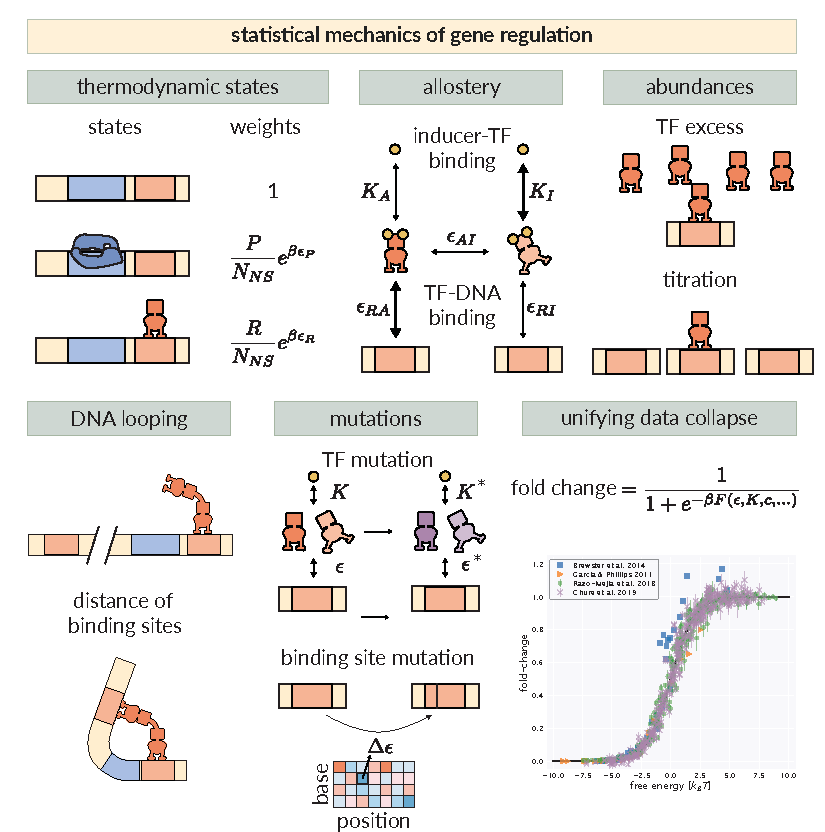
\includegraphics[width=\textwidth]{figures/intro/stat-mech_gene-regulation.pdf}
\caption[statmech]{\textbf{statmech}}\label{fig:statmech}
\index{figures}
\end{figure}


\indent This vast set of parameters accumulates in a powerful data collapse, where data from experiments of diverse perturbations collapse on a single curve, unifying many different aspects of gene regulation into a single, predictive theory. It highlights the universality of the underlying Boltzmann distribution; whether binding affinities or copy numbers are changed, the model of gene regulation obeys the same thermodynamic master curve. The existence of such a curve demonstrates that our understanding of these systems has reached a point where we are no longer merely describing biological phenomena, but predicting them from first principles. By knowing the DNA sequence and the protein concentrations, we can accurately calculate the census of RNA polymerase on a promoter and, by extension, the physiological state of the cell.

\indent While the majority of these regulatory motifs are well-described by the "passive" occupancy models of thermodynamic equilibrium, recent work has explored how the cell adds layers of sophistication through energy-consuming processes. As shown in Figure~\ref{fig:graphs}, by allowing certain transition rates to break detailed balance—often through the hydrolysis of ATP—the cell can achieve non-monotonic dose-response curves or ultra-sensitive switches that exceed the limits of equilibrium models~\citep{mahdavi2024flexibility}. Rather than contradicting the thermodynamic framework, these non-equilibrium models represent the "fine-tuning" of an already robust system, allowing for a level of regulatory flexibility that matches the complexity of the environments in which these bacteria thrive.
\begin{figure}[hbt!]
\centering
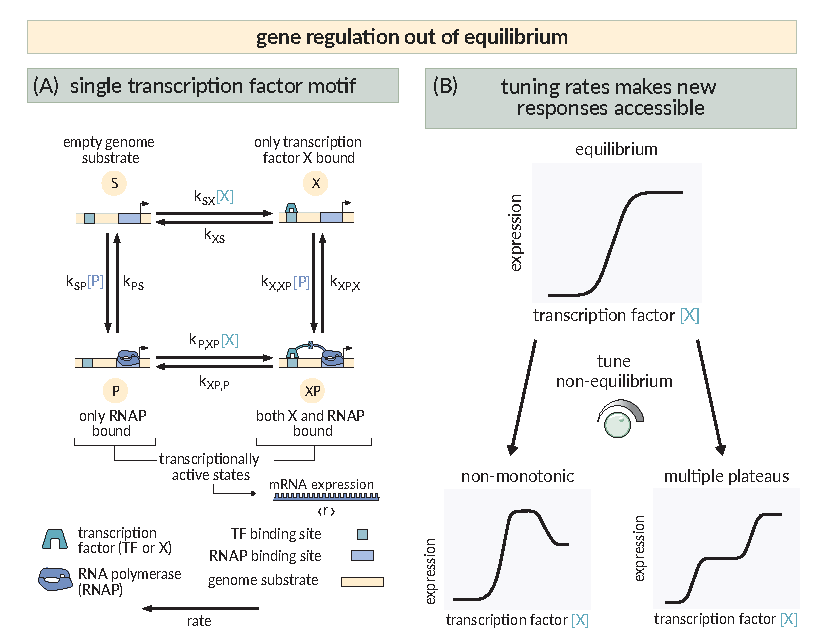
\includegraphics[width=\textwidth]{figures/intro/graphs.pdf}
\caption[graphs]{\textbf{Non-equilibrium gene regulation via graph theory.} (A) A four-state cycle representing a single transcription factor regulating a promoter. In equilibrium models, transition rates satisfy detailed balance. (B) By relaxing the equilibrium assumption and introducing energy-consuming transitions (e.g., via ATP hydrolysis), the system can achieve complex regulatory behaviors, such as intermediate plateaus or non-monotonic dose-response curves, which are inaccessible to standard thermodynamic models. Adapted from \cite{mahdavi2024flexibility}}\label{fig:graphs}
\index{figures}
\end{figure}

\indent In summary, the study of gene regulation in \textit{E. coli} has evolved from the discovery of logical switches to a comprehensive biophysical theory. We now possess a detailed map of how molecular geometry, DNA sequence, and protein-protein interactions converge to control the flow of genetic information with remarkable precision.

\section{Genomic dark matter}
Why is there nothing here

\section{The Era of Sequencing}
\noindent In todays age, the 2020s, DNA sequencing has become a technique so ubiquitous, it has infiltrated many corners of our lives beyond the natural sciences, such as paternity test, ancestry tests and criminal investigations. Sequencing data is being generated at will in amounts that were unimaginable just two decades ago. 
\begin{itemize}
    \item data explosion
    \item sequencing without genomes
    \item sanger sequencing 
    \item 2nd gen sequencing 
    \item third gen sequencing
    \item RNA sequencing with a reference\citep{mortazavi2008mapping}
\end{itemize}



\section{Discovery of DNA binding sites}
\begin{itemize}
    \item gel mobility assay 
    \item  
\end{itemize}
\section{Description of chapters}
\begin{itemize}
    \item HERNAN seq
    \item Description of Reg-Seq experiment and summary statistics
    \item Data Processing of Reg-Seq
    \item Identification of binding sites
    \item De novo promoters
    \item other interesting results
    \item Future experiments
    \item 
    \item 
\end{itemize}

\printbibliography[heading=subbibliography]
\end{refsection}


\appendix

\chapter{Questionnaire}
\chapter{Consent Form}

\printindex

\theendnotes
\end{document}
